\documentclass[tikz, convert={outfile=\jobname.png}]{standalone}
\usepackage{amsmath,tikz}
\usepackage{xcolor}
\usetikzlibrary{backgrounds,calc}
\usepackage{tikz-3dplot}
\begin{document}



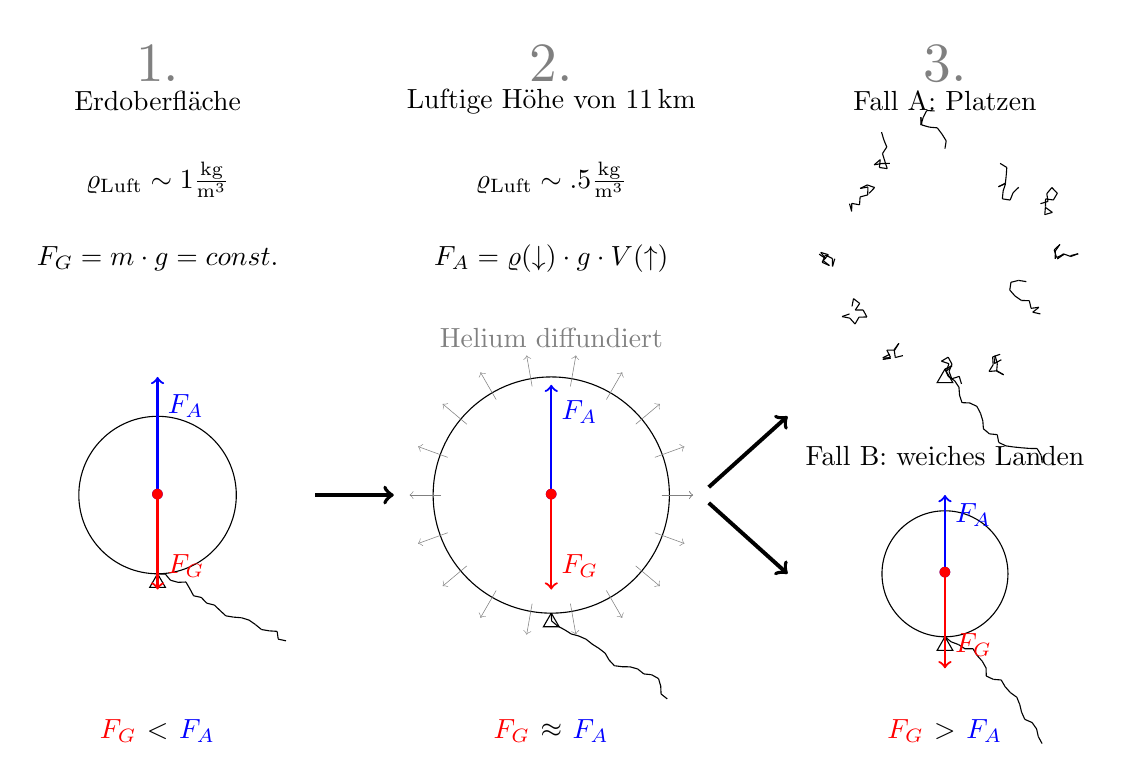
\begin{tikzpicture}

%%Erdoberfläche
\path(0,5)node{Erdoberfl\"ache}node[above,scale=2,gray]{1.};
\path(0,4)node{$\varrho_{\textnormal{Luft}} \sim 1 \frac{\textnormal{kg}}{\textnormal{m}^3}$};
\draw (0,0)circle(1)++(0,-1)--++(240:.2)--++(0:.2)--++(120:.2)coordinate(A);
\foreach \i in {1,2,...,20}{\draw[rounded corners=2pt] (A)--++(270+rnd*100:.1)coordinate(A);}

\draw[->,thick,blue] (0,0)node{$\bullet$}--++(0,1.5)node[near end,right]{$F_{A}$};
\draw[->,thick,red] (0,0)node{$\bullet$}--++(0,-1.2)node[near end,right]{$F_{G}$};
\path(0,3)node{$F_G = m \cdot g = const.$};
\path(-.5,-3)node[red]{$F_G$};
\path(0,-3)node[]{$<$};
\path(.5,-3)node[blue]{$F_A$};

\draw[line width=.05cm,->] (2,0)--(3,0);

%% Luftige Höhe
\path(5,5)node{Luftige H\"ohe von 11\,km}node[above,scale=2,gray]{2.};
\path(5,4)node{$\varrho_{\textnormal{Luft}} \sim .5 \frac{\textnormal{kg}}{\textnormal{m}^3}$};
\path(5,3)node{$F_A = \varrho (\downarrow) \cdot g \cdot V(\uparrow)$};
\draw (5,0)circle(1.5)++(0,-1.5)--++(240:.2)--++(0:.2)--++(120:.2)coordinate(A);
\foreach \i in {1,2,...,20}{\draw[rounded corners=2pt] (A)--++(270+rnd*100:.1)coordinate(A);}

\draw[->,thick,blue] (5,0)node{$\bullet$}--++(0,1.4)node[near end,right]{$F_{A}$};
\draw[->,thick,red] (5,0)node{$\bullet$}--++(0,-1.2)node[near end,right]{$F_{G}$};
\foreach \n in {0,20,...,360}{\draw[help lines, very thin,->,xshift=5cm] (\n:1.4)--(\n:1.8); }
\path[help lines, very thin](5,2)node{Helium diffundiert};

\draw[line width=.05cm,->] (7,.1)--(8,1);
\draw[line width=.05cm,->] (7,-.1)--(8,-1);



\path(5-.5,-3)node[red]{$F_G$};
\path(5,-3)node[]{$\approx$};
\path(5.5,-3)node[blue]{$F_A$};

%% Platzen
\path(10,5)node{Fall A: Platzen}node[above,scale=2,gray]{3.};
\draw (10,3)coordinate(B)++(0,-1.4)--++(240:.2)--++(0:.2)--++(120:.2)coordinate(A);
\foreach \i in {1,2,...,20}{\draw[rounded corners=2pt] (A)--++(270+rnd*100:.1)coordinate(A);}

\foreach \n in {0,30,...,330}{
\path (10,3)++(\n:1.4)coordinate(A);
\foreach \i in {1,2,...,10}{
\draw[xshift=10cm,yshift=3cm] (A)--++(\n+40+rnd*360:.1)coordinate(A);
}}


%% Landen

\draw (10,-1)circle(.8)++(0,-.8)--++(240:.2)--++(0:.2)--++(120:.2)coordinate(A);
\foreach \i in {1,2,...,20}{\draw[rounded corners=2pt] (A)--++(270+rnd*100:.1)coordinate(A);}

\path(10-.5,-3)node[red]{$F_G$};
\path(10,-3)node[]{$>$};
\path(10.5,-3)node[blue]{$F_A$};


\draw[->,thick,blue] (10,-1)node{$\bullet$}--++(0,1)node[near end,right]{$F_{A}$};
\draw[->,thick,red] (10,-1)node{$\bullet$}--++(0,-1.2)node[near end,right]{$F_{G}$};

\path(10,.5)node{Fall B: weiches Landen};


\end{tikzpicture}

\end{document}